\documentclass[11pt]{article}
\usepackage[pdftex]{graphicx}
\usepackage[utf8]{inputenc}
\usepackage{float}										% positioning of floats such as graphics, tables
\usepackage{subfig}
\usepackage{amsmath}									% advanced math extensions
\usepackage{latexsym}									% other mathematical symbols
\usepackage{amssymb}									% other mathematical symbols
\usepackage{amsthm}										% theorem environment
%\usepackage{commath}									% differential operators \dif
\usepackage{mathrsfs}									% mathscr font in math mode																
\usepackage{setspace}									% modifiable line pitch
\usepackage{array}										% extends possibility of LaTeX to handle tables
\usepackage{hyperref}									% best package wo je h�ts gits
\usepackage{parskip}									% no indention for new paragraphs
\usepackage{framed}										% framed environment for framed text
\usepackage{fancyhdr} 									% change header and footer of any page of the document
\usepackage{mdwlist}									% smaller line pitch for \itemize, \enumerate
\usepackage{color}										% adds support for colored text
\usepackage[english]{babel}
\usepackage{tikz}										% nice drawing environment
\usetikzlibrary{arrows}
\usetikzlibrary{positioning}

\renewcommand{\labelitemi}{--}
\newcommand{\unit}[1]{\ensuremath{\, \mathrm{#1}}}			% units

\definecolor{darkblue}{rgb}{0,0,.4}
\definecolor{darkgreen}{rgb}{0,0.5,0}
\hypersetup{pdfborder={0 0 0},colorlinks=true,linkcolor=darkblue,citecolor=darkgreen}


\newcommand{\lint}{\mathlarger{\int}}
\newcommand{\R}{\mathbb{R}}
\newcommand{\C}{\mathbb{C}}
\newcommand{\N}{\mathbb{N}}
\newcommand{\Z}{\mathbb{Z}}
\newcommand{\Q}{\mathbb{Q}}
\newcommand{\linspan}{\operatorname{span}}
\newcommand{\nextpar}{\vspace{5pt}}
\newcommand{\type}{~\mathtt}

\newcommand{\HRule}{\rule{\linewidth}{0.5mm}}
\usepackage[a4paper,left=2.5cm, right=2.5 cm, top=2.5cm, bottom=2cm]{geometry}


\usepackage{pdfpages}

\pagestyle{fancy}
\fancyhead{}
\fancyfoot{} 
\fancyhead[L]{\sffamily  {\small FastCode}}
\fancyhead[R]{\sffamily  {\small Homework 5}}

\setlength\extrarowheight{5pt}
\begin{document}
\hspace{0.2 in}
\begin{center}
	\begin{Large}
		\textbf{Homework 5: Solutions Dominik Gresch}
	\end{Large}
\end{center}
\subsection*{Exercise 1: Mini-MMM}
	The system used for this exercise is an Intel Core i7-4700MQ @ 2.4 $\unit{GHz}$ \\(32 \unit{kB} L1 cache, 256 \unit{kB} L2 cache, ADD tp 1, MUL tp 2)
	\begin{itemize}
		\item[a) - d)] The files can be found in \texttt{impl/src/} 
		\item[e)] The working set fits into cache if
			\[ \left\lceil \frac{N_B^2}{B_1} \right \rceil +  3 \cdot \left \lceil \frac{N_B\cdot M_U}{B_1} \right \rceil + \left \lceil \frac{M_U \cdot N_U}{B_1} \right\rceil \leq \frac{C_1}{B_1}  \]
			
			This gives $N_B \leq 87$ for \texttt{code1} and \texttt{code2} (which has to be rounded to $N_B = 86$) and $N_B = 88$ for \texttt{code3} (see calculations in the \texttt{Mathematica} file).\\
			I get the following results:
			\begin{figure}[H]\centering
				\begin{tabular}{l|l}

				version & performance $[\mathtt{\frac{flop}{cycle}}]$\\\hline
				\texttt{code1} & 0.86 \\
				\texttt{code2} & 1.44 \\
				\texttt{code3} & 1.30
				\end{tabular}
			\end{figure}
			It turns out that \texttt{code2} is by far the fastest.
		\item[f)] Now, we get $N_B \leq 177$ for \texttt{code1} and \texttt{code2} (round to $N_B = 176$) and $N_B \leq 179$ (round to $N_B = 176$) for \texttt{code3}.
		\begin{figure}[H]\centering
			\begin{tabular}{l|l}	
				version & performance $[\mathtt{\frac{flop}{cycle}}]$\\\hline
				\texttt{code1} & 0.86 \\
				\texttt{code2} & 1.18 \\	
				\texttt{code3} & 1.18
			\end{tabular}
		\end{figure}
		Amongst those versions, \texttt{code2} is again the fastest (on par with \texttt{code3}, within error). Overall, however, \texttt{code2} for $N_B = 86$ gives the best performance.
	\end{itemize}
	\newpage
\subsection*{Exercise 2: MMM}
	\texttt{finalcode.c} can again be found in \texttt{impl/src/}
	\begin{figure}[H]\centering
		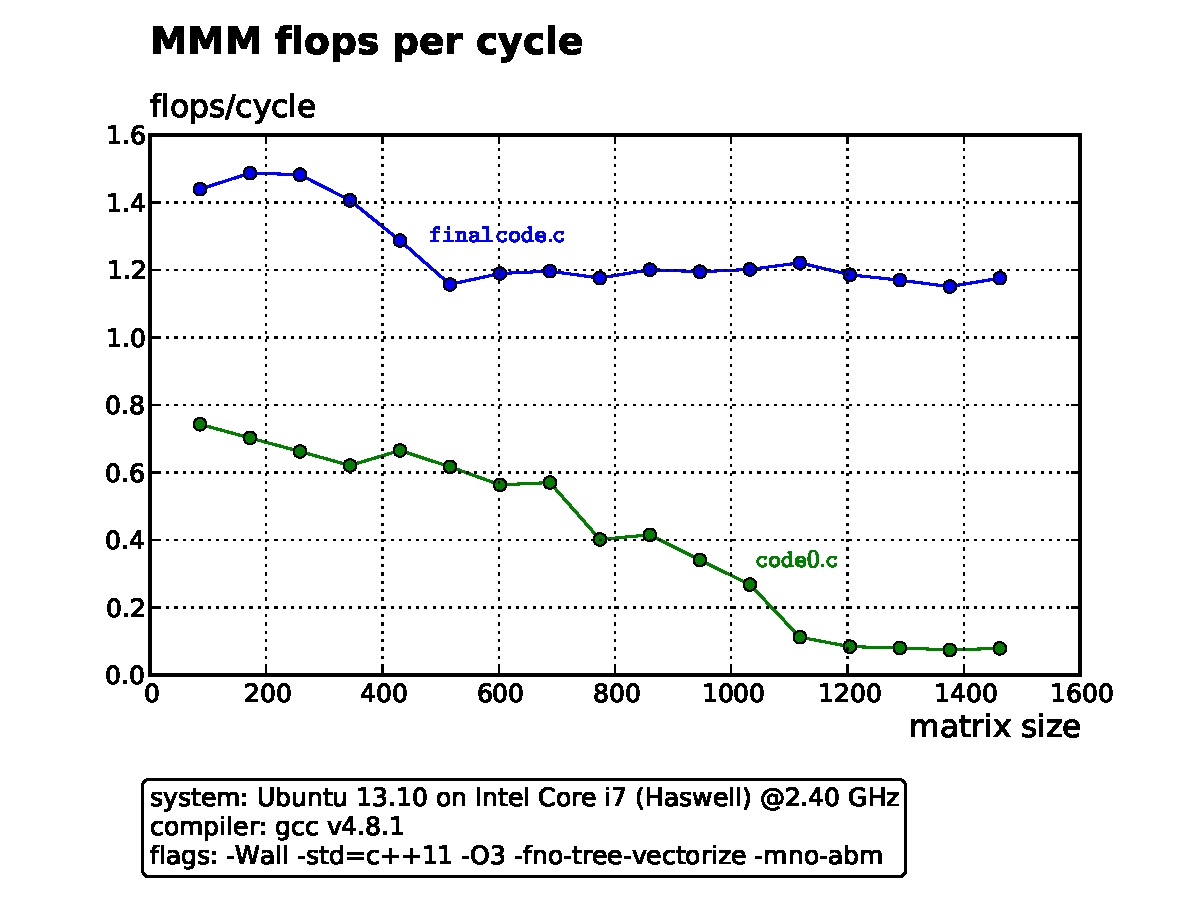
\includegraphics[width = 6in]{performance.pdf}
	\end{figure}

\subsection*{Exercise 3: Roofline}
	\begin{itemize}
		\item[a)] The processor can issue 2 mults and 1 add per cycle, hence the peak performance is
		\[ \Rightarrow \pi = 3 \type{\frac{flop}{cycle}} \]
		\item[b)] The maximum bandwith is $25.6 \unit{GB \cdot s^{-1}}$ at a frequency of $3.2 \unit{GHz}$. This means the maximum bandwidth is
		\[ \beta = \frac{25.6}{3.2} \type{\frac{byte}{cycle}} = 8 \type{\frac{byte}{cycle}}  \]
		\item[c)] MMM cannot reach peak performance on this system, because the flops are not balanced: There are equally many additions and multiplications, whereas the processor can issue twice as many multiplications as additions. Therefore the maximum performance for MMM is limited by the throughput of ADD, i.e. only one multiplication can actually be issued per cycle (limited by the dependency on the adds).\\
		The performance of MMM is hence limited by 
		\[ \pi' = 2 \type{\frac{flop}{cycle}} \]
		\item[d)]
		For \texttt{fjump(x, 3*1024*1024)}, the computation is memory bound:\\
		For each iteration in \texttt{i}, at least $\frac{3\cdot1024\cdot1024}{16} \cdot 64 \type{byte} = 12 \type{MB}$ of data are read (one cacheline containing \texttt{x[j]} and \texttt{x[j+1]}; the \texttt{x} for the next \texttt{j}-iteration cannot be on the same cacheline).\\
		Since the LLC is only $6 \type{MB}$, this means that access to \texttt{x[j]} will always be a miss. Accessing \texttt{x[j+1]} will be a hit as long as it is on the same cacheline as \texttt{x[j]} (this depends on the alignment of \texttt{x}). A hard lower bound for Q is 
		\[ Q \geq 16 \cdot 12 \type{MB} =  192 \type{MB} \] 
		Which can be used to find an upper bound for the operational intensity:
		\[ W = 2 \cdot 3 \cdot 1024 \cdot 1024 \type{flop} = 6 \type{Mflop} \Rightarrow I \leq \frac{6}{192} \type{\frac{flop}{byte}} = \frac{1}{32} \type{\frac{flop}{byte}} \]
		This then gives a tighter bound for the performance: 
		\[ \pi'' \leq \beta \cdot I = \frac{1}{4} \type{\frac{flop}{cycle}}  \]
		\begin{figure}[H]\centering
			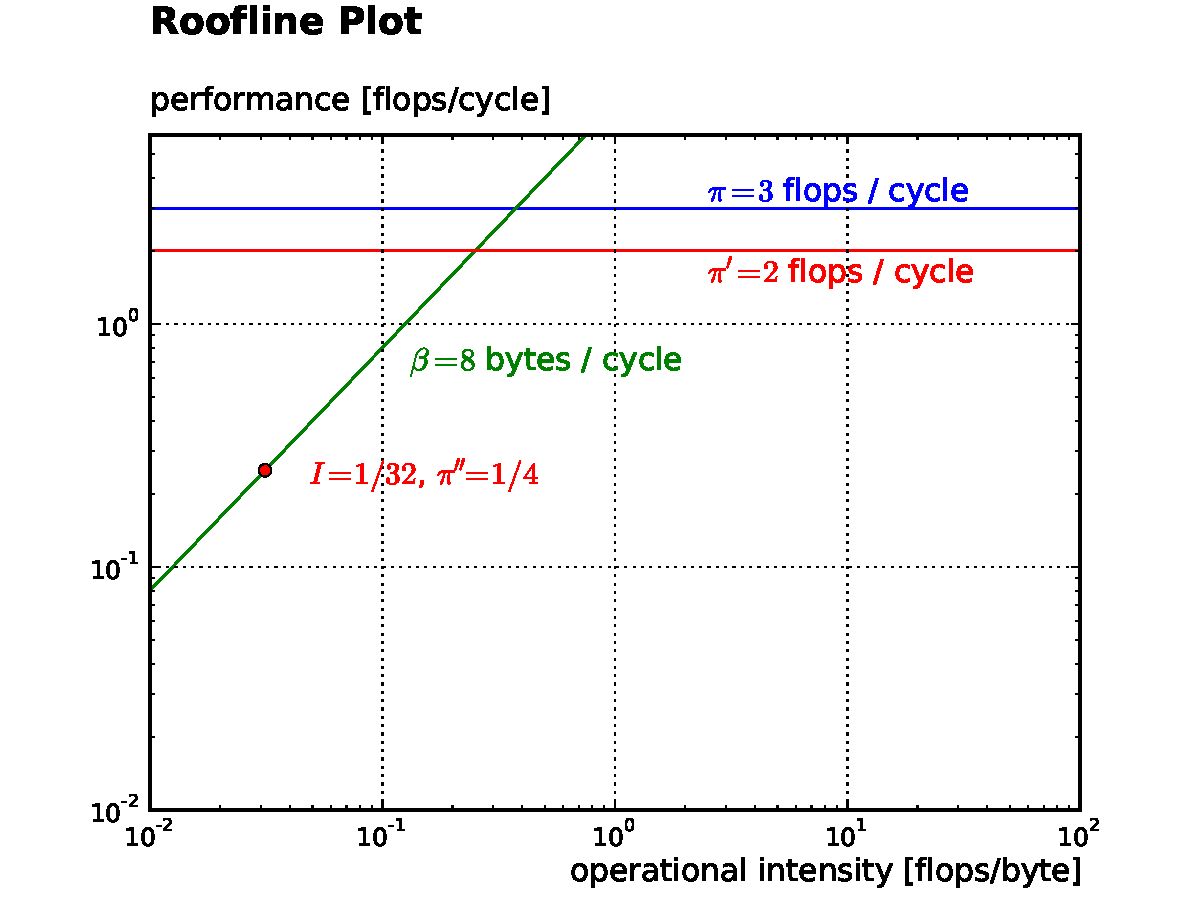
\includegraphics[width = 6 in]{roofline.pdf}
		\end{figure}
	\end{itemize}
\end{document}